Nodes for wireless sensor networks have been created in the past \cite{voinescu2013lightweight}, V3.2 is a successful
iteration based on Atmel Atmega128RFA1. Paired with the node, a dongle can be connected to a
computer using an USB port which allows the PC to act as a gateway for the network of nodes. Even
though the node is very low power, developing new applications on the node is very complicated. The
only way to program a node is using an ISP programmer using a dautgher board that contains a JTAG
and ISP connector and a FTDI for usb to serial connection. Adding new hardware is very difficult, the expansion
capabilities are limited which leads to using only the existing sensors mounted on the node.

\begin{figure}[ht] \centering
\includegraphics[width=0.5\textwidth]{img/sparrowv32.jpg}
\caption{Sparrow V3.2 with gateway and programming base board}
\end{figure}


The next iteration, the Sparrow V4 based on the same microcontroller as Sparrow V3.2, tried to fix
the development environment by being Arduino \cite{arduino}
compatible. This removed ISP programming, but it is still necessary to use the extensions daughter board
with FTDI in order to program the board. The limited expansion capabilities are still an issue and, unfortunately, the node
has a very high power consumption of between 400uA up to 1.5mA \cite{geo} when in deep sleep.

Another problem is that Sparrow is directly powered from an external source, which we must make
sure it is between 1v8 and 3v6, depending on the sensors maximum operating voltage, otherwise there
is a possibility that some components might be destroyed. Because the
microcontroller has an internal LDO, it will have the same current consumption regardless of the
operating voltage resulting in the power consumption to vary between 7.4mW up to 14.8mW for the cpu
and between 32.5mW up to 65mW when transmitting data. Also, the power for on-board sensors is cut
using an mosfet-N on the common GND line. Due to this, some sensors can "borrow" the GND from
digital pins which increases the power consumption.
\begin{figure}[ht] \centering
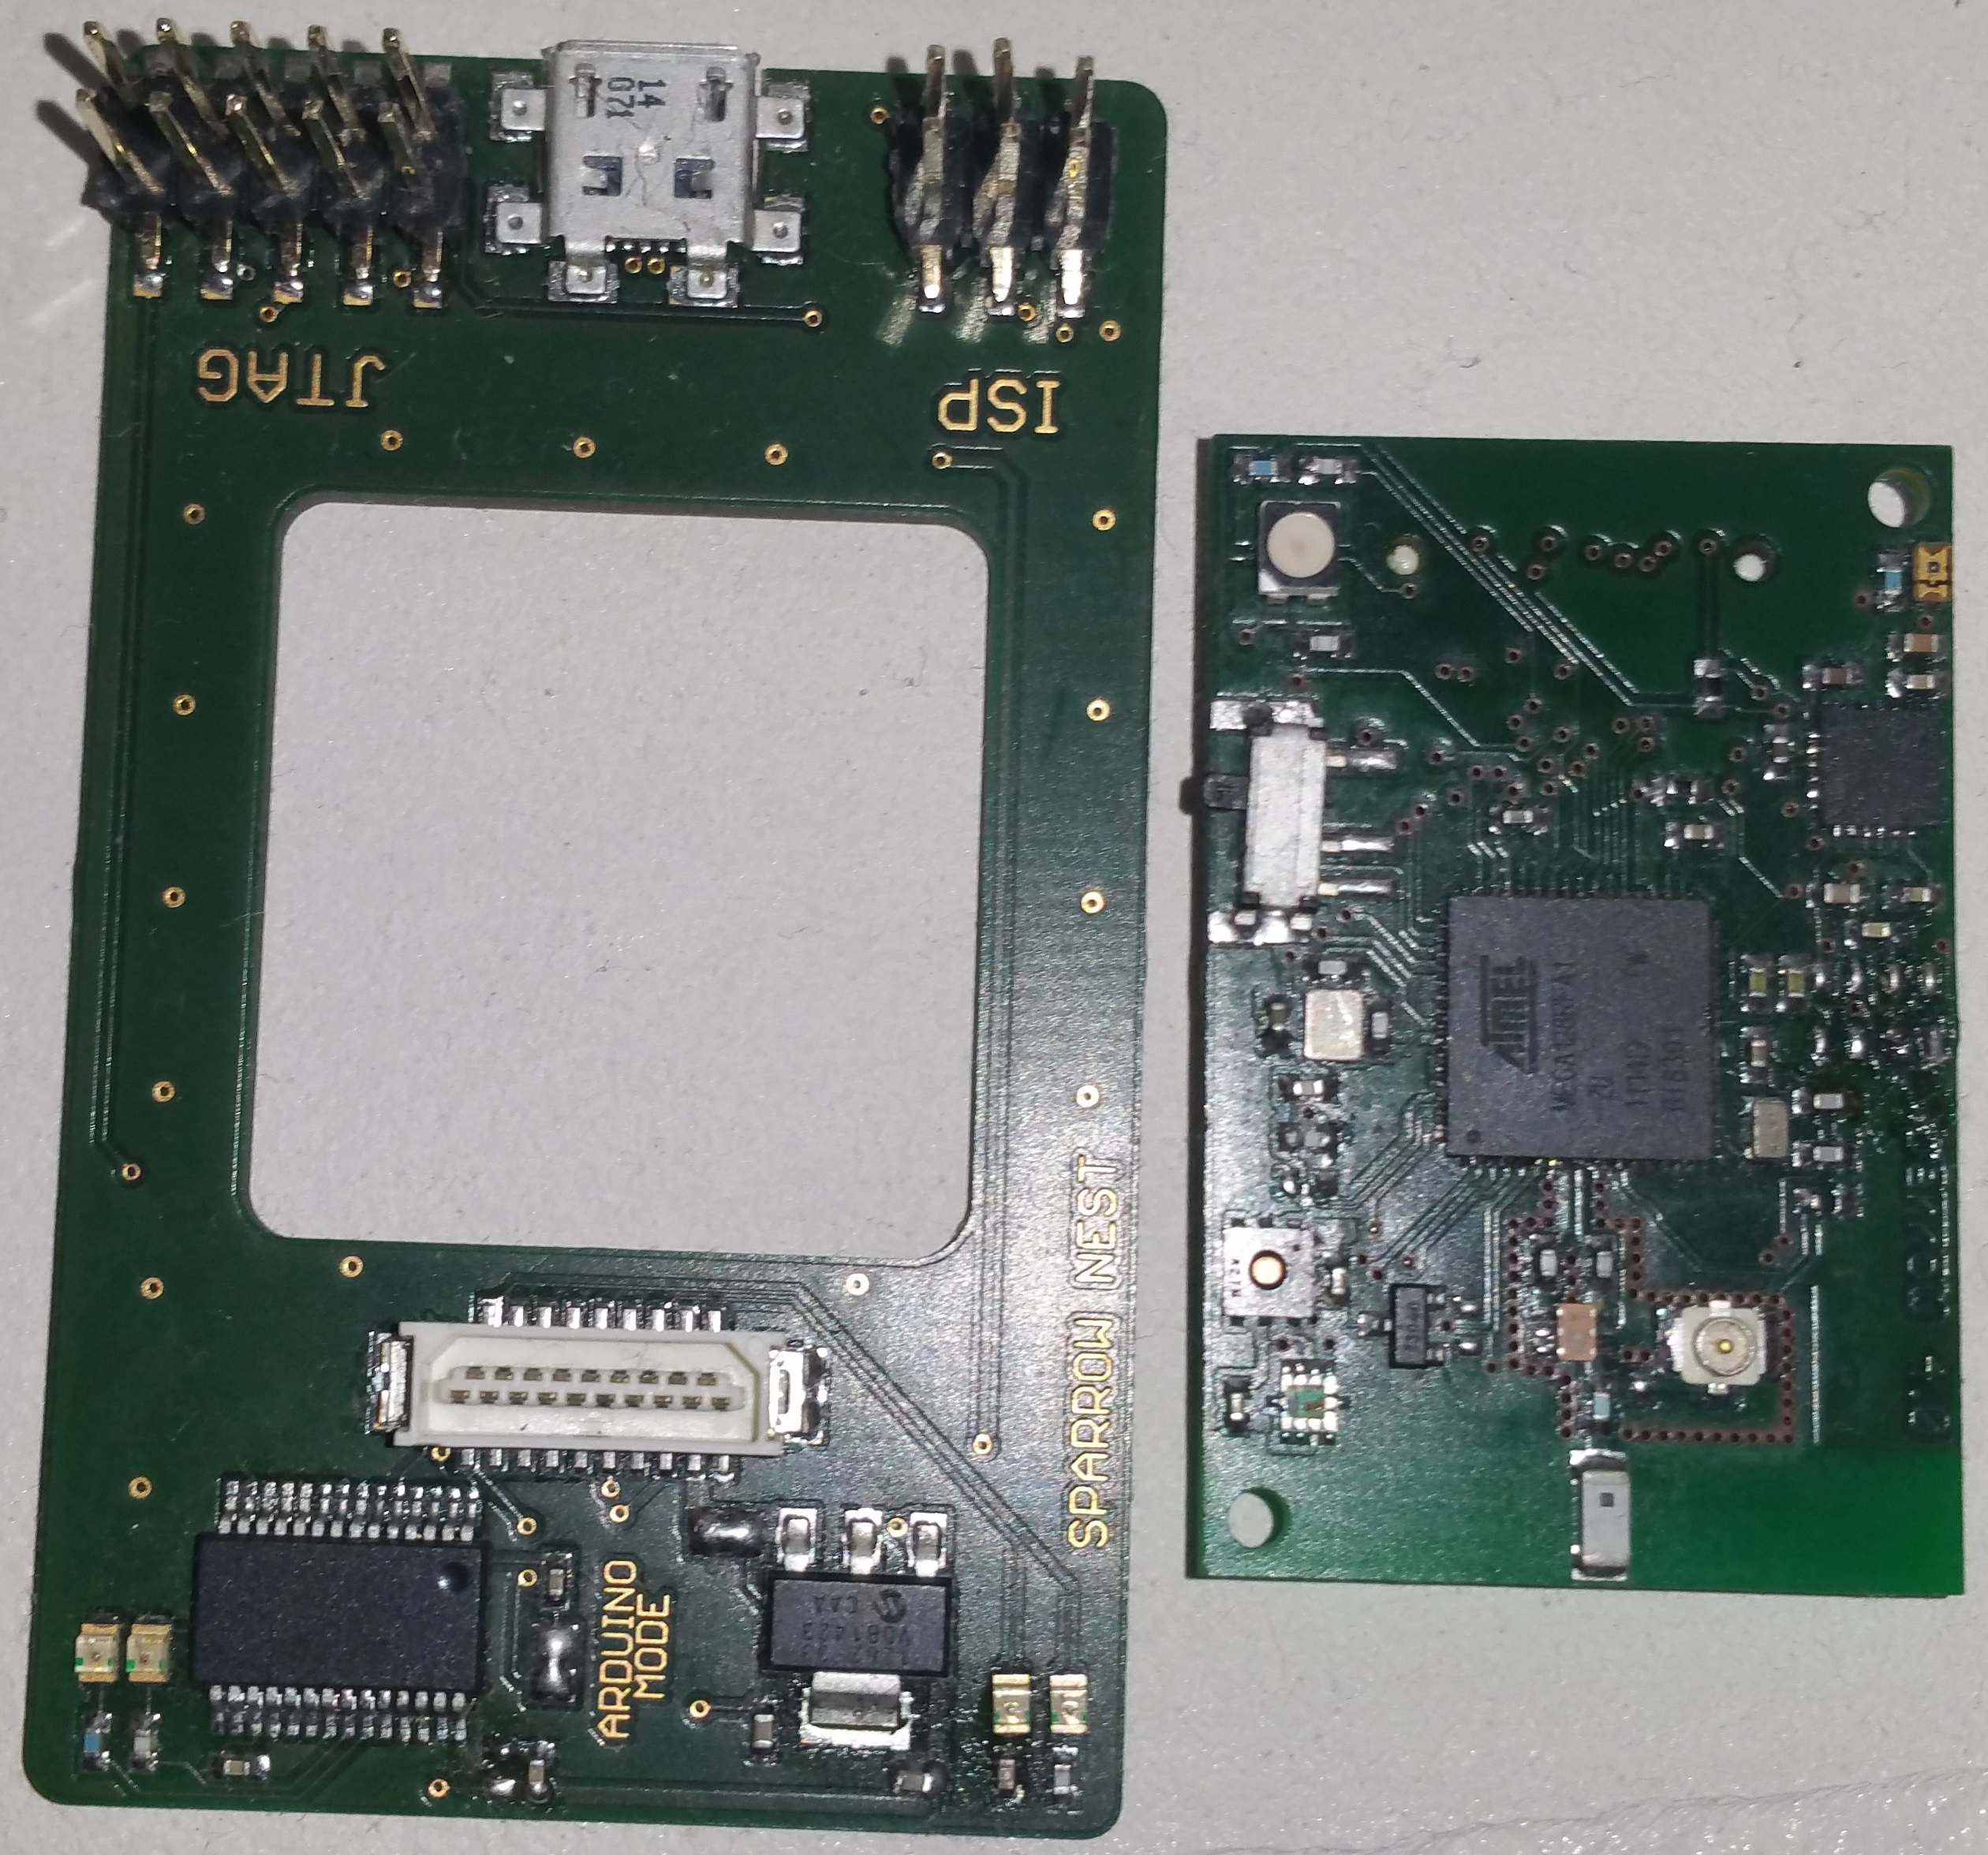
\includegraphics[width=0.5\textwidth]{img/sparrowv4.jpg}
\caption{Sparrow V4 with programming base board}
\end{figure}



